\chapter{Konzeption}
\label{chapter4}
Vor der eigentlichen Implementierung erfolgt nun eine ausführliche Konzeption.
Diese dient dazu genau zu elaborieren, welche Anforderungen an die Software gestellt werden
und wie die Implementierung erfolgen soll.
Etwaige Ungereimtheiten und Probleme können so frühzeitig erkannt werden.


\section{Anforderungsanalyse}
\label{4-Anforderungsanalyse}
Es soll ein System implementiert werden,
welches Kinect-Bewegungsdaten mithilfe von hierarchischem Clustering
und \ac{DTW} als Distanzmetrik gruppiert.
Dieses Tool kann im Rahmen des HoPE-Projekts genutzt werden,
um große Datensätze auf wiederkehrende Bewegungsabläufe bei der Interaktion mit Wandbildschirmen
zu untersuchen.
Dabei gibt es sogenannte \emph{funktionale Anforderungen} und \emph{nicht-funktionale Anforderungen},
die das System erfüllen muss.
Letztere beinhalten beispielsweise Anforderungen zu Benutzbarkeit, Effizienz oder Portierbarkeit.
Funktionale Anforderungen beschreiben hingegen die primären Features des Systems.

\subsection{Nicht-funktionale Anforderungen}
\label{4-NichtFunktionaleAnforderungen}
Bei der Wahl der genutzten Programmiersprache und möglicherweise verwendeten Frameworks
existieren keine speziellen Vorgaben.
Das Tool sollte allerdings ohne großen Installationsaufwand nutzbar sein
und daher nach Möglichkeit eine stark verbreitete Programmiersprache nutzen.
An die Effizienz gibt es ebenfalls keine besonderen Anforderungen,
da die Auswertung der Daten nur einmalig zu einem späteren Zeitpunkt erfolgt.
Eine Echtzeitauswertung ist nicht geplant.
Das Tool sollte durch wenige Anpassungen auch auf Datensätze anderer Tiefenkameras angewandt werden können.
Um dieses Ziel zu erreichen, wird die Software von Beginn an möglichst generisch entwickelt.

\subsection{Funktionale Anforderungen}
\label{4-FunktionaleAnforderungen}
Die Software bietet Input-Funktionalitäten,
mit der ein Datensatz aus Textdateien eingelesen und in passenden Datenobjekten abgespeichert werden kann.
Das Tool soll ein Clustering mittels hierarchischem Clustering wie in \autoref{3-Clustering} beschrieben anbieten.
Dabei ist der Threshold für das Mergen von zwei Clustern vom Nutzer konfigurierbar.
Als Distanzmetrik wird \ac{DTW} (\autoref{3-DTW}) genutzt.
Dabei ist konfigurierbar, welche Attribute des Datensatzes für den Vergleich genutzt werden.
Zudem besitzt die Implementierung Output-Funktionalitäten.
Die gefundenen Cluster werden in einer Textdatei aufgelistet.
Jedes Cluster erhält einen eindeutigen Namen und eine Liste aller Records die zusammengeführt wurden.
Die starke Konfigurierbarkeit wird durch eine \emph{config-file} erreicht,
die der Nutzer beim Start der Anwendung übergeben kann.
Sie enthält unter anderem ein \emph{keywort} welcher Datensatz verwendet wird (z.B. \glqq kinect\grqq),
den Pfad zum Datensatz, die zu nutzendem Attribute für den Vergleich des \ac{DTW}-Algorithmus,
den Threshold für das Clustering und den Pfad zur Output-Datei.

\section{Programmablauf}
\label{4-Programmablauf}
Im Folgenden wird ein typischer Programmablauf beschrieben.
\begin{enumerate}
    \item Der Nutzer startet den \emph{Clustering-Processor} und gibt als Startparameter den Pfad der config-Datei an.
    \item Der \emph{Processor} nutzt den \emph{Config-Reader}, um die Werte der Konfigurationdatei auszulesen
    und speichert diese ab.
    \item Der \emph{Processor} nutzt den \emph{TS-Reader}, um den Datensatz einzulesen
    und legt die Informationen in geeigneten Objekten ab.
    Beim Kinect-Datensatz sind das \emph{KinectRecord} und \emph{KinectFrame}.
    \item Der \emph{Processor} startet das Clustering durch den Aufruf der \emph{cluster-Methode}
    der \emph{HierarchicalClustering-Klasse}.
    Zu beginn entspricht jeder Record einem eigenen Cluster.
    Die \emph{recordToCluster-Methode} ermöglicht eine Transformation.
    \item Das Clustering nutzt die \emph{\ac{DTW}-Implementierung},
    um paarweise die Kosten zwischen zwei Clustern zu berechnen.
    \item Die beiden Cluster mit den geringsten Kosten werden zusammengeführt.
    Dazu wird ein neues \emph{Cluster-Objekt} angelegt, dass durch Kombination der beiden Cluster entsteht.
    In diesem Cluster werden die Bestandteile (Records, Cluster) abgespeichert.
    Bei allen Komponenten wird ein \emph{consider-flag} auf \emph{false} gesetzt,
    damit sie bei zukünftigen Vergleichen nicht mehr berücksichtigt werden.
    \item Schritte 5 und 6 so lange wiederholen, bis die geringsten Kosten den vom Nutzer definierten Threshold übersteigen.
    \item Der \emph{Processor} nutzt den \emph{Cluster-Writer}, um alle Cluster der \emph{clusters-Liste}
    in eine Ausgabedatei zu schreiben.
    \item Die Anwendung terminiert. 

\end{enumerate}


\section{Teilsysteme}
\label{4-Teilsysteme}
ToDo.

\begin{figure}[ht]
    \begin{center}
    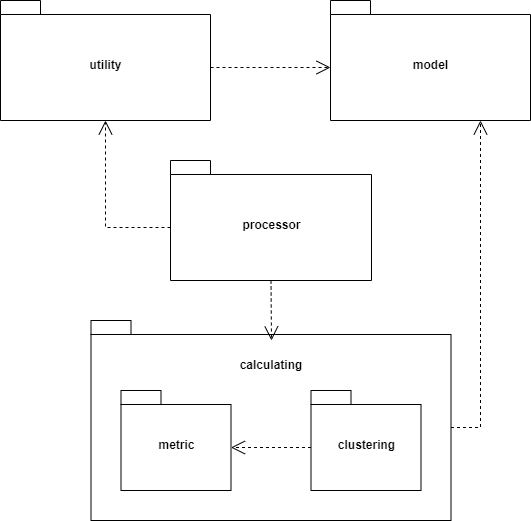
\includegraphics[width=\textwidth]{packages.png}
    \end{center}
    \caption{Vorläufiges Paketdiagramm.}
    \label{fig:Packages}
\end{figure}

\begin{figure}[ht]
    \begin{center}
    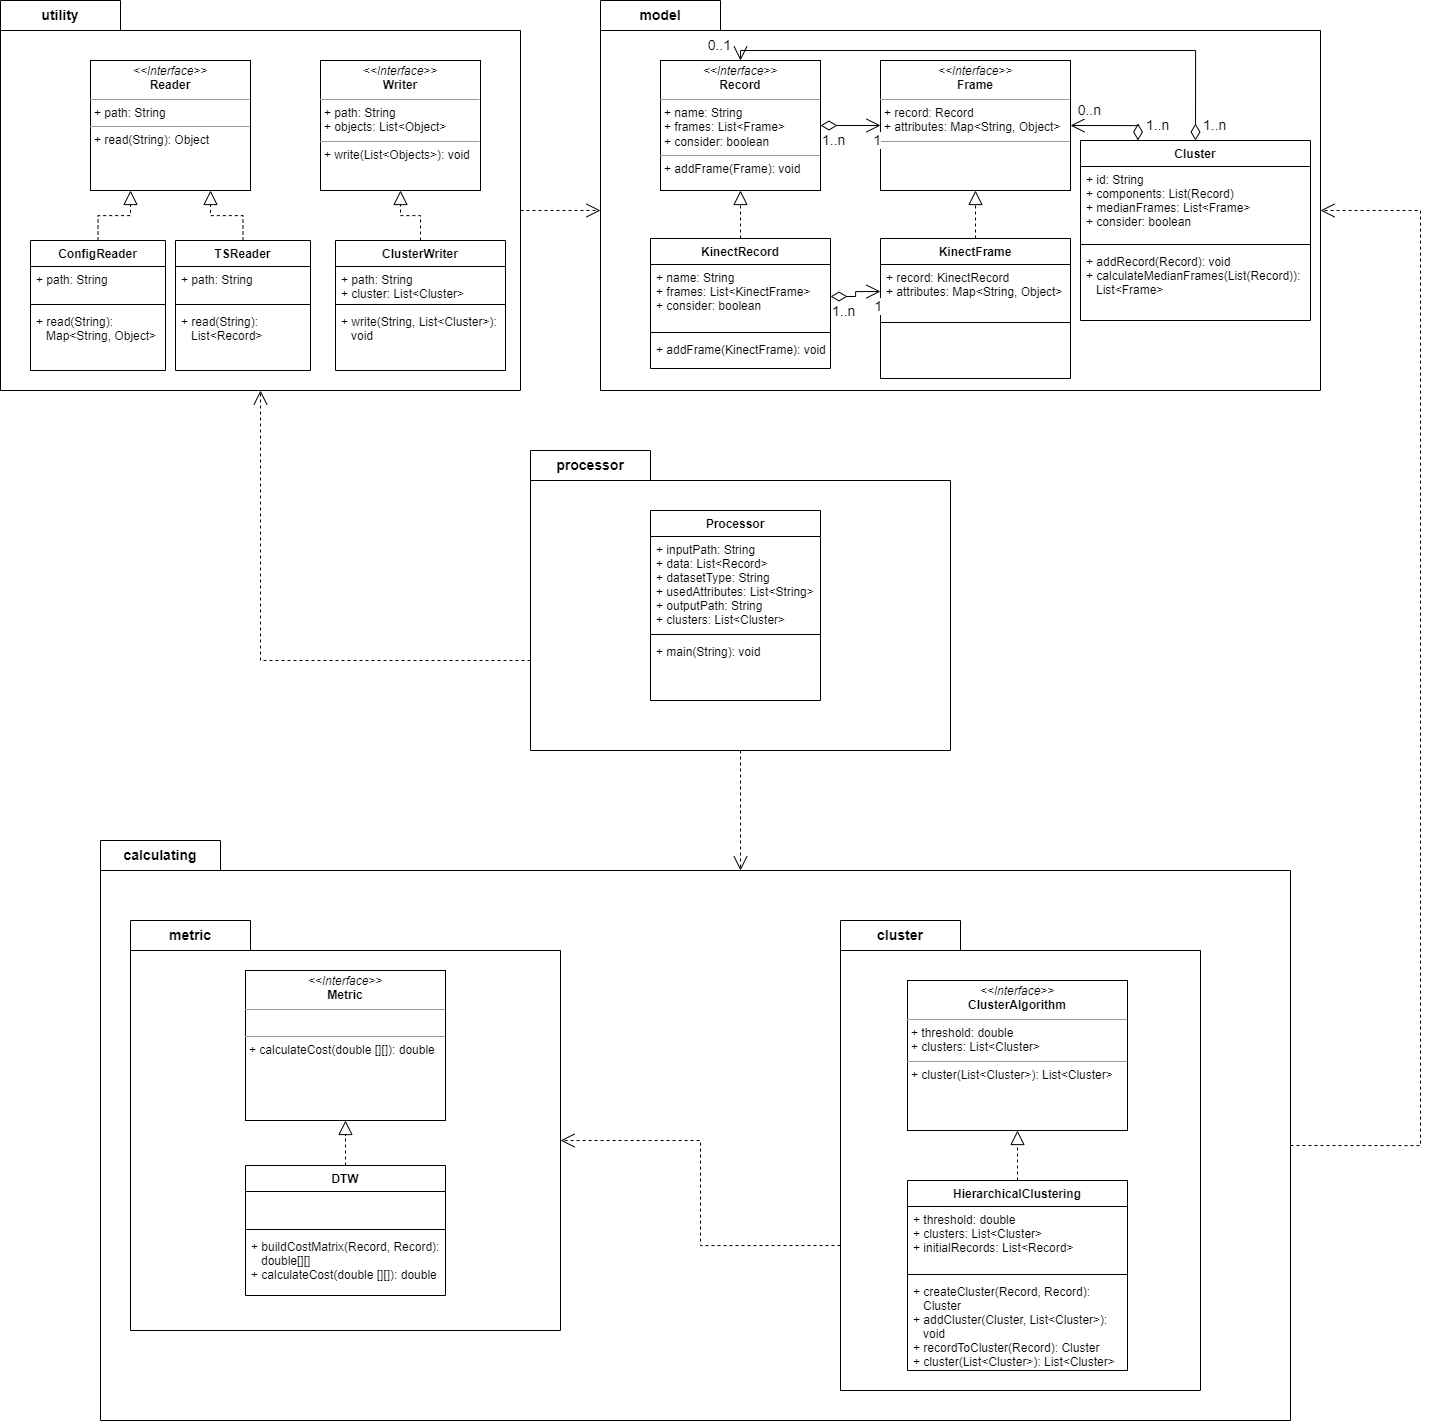
\includegraphics[width=\textwidth]{classes.png}
    \end{center}
    \caption{Vorläufiges Klassendiagramm.}
    \label{fig:Classes}
\end{figure}
